% ----------------------- TODO ---------------------------
%Template 
\documentclass[a4paper]{scrartcl}
\usepackage[utf8]{inputenc}
%\usepackage[ngerman]{babel}
\usepackage{geometry,forloop,fancyhdr,fancybox,lastpage}
\usepackage{listings}
\lstset{frame=tb,
	language=Java,
	aboveskip=3mm,
	belowskip=3mm,
	showstringspaces=false,
	columns=flexible,
	basicstyle={\small\ttfamily},
	numbers=left,
	numberstyle=\tiny\color{gray},
	keywordstyle=\color{blue},
	commentstyle=\color{dkgreen},
	stringstyle=\color{mauve},
	breaklines=true,
	breakatwhitespace=true,
	tabsize=3
}
\geometry{a4paper,left=3cm, right=3cm, top=3cm, bottom=3cm}
% Diese Daten müssen pro Blatt angepasst werden:
\newcommand{\NUMBER}{4}
\usepackage{graphicx}
%\graphicspath{{maps/}}
\newcommand{\EXERCISES}{5}
% Diese Daten müssen einmalig pro Vorlesung angepasst werden:
\newcommand{\COURSE}{Methoden der Algorithmik}
%\newcommand{\TUTOR}{Benjamin Coban}
\newcommand{\STUDENTA}{Stefan Wezel}
\newcommand{\STUDENTB}{Lukas Günthner}
%\newcommand{\STUDENTC}{Gwent Krause}
\newcommand{\DEADLINE}{\date}
% ----------------------- TODO ---------------------------



%Math
\usepackage{amsmath,amssymb,tabularx}

%Figures
\usepackage{graphicx,tikz,color,float}
\graphicspath{ {home/stefan/picures/} }
\usetikzlibrary{shapes,trees}

%Algorithms
\usepackage[ruled,linesnumbered]{algorithm2e}

%Kopf- und Fußzeile
\pagestyle {fancy}
%\fancyhead[L]{Tutor: \TUTOR}
\fancyhead[C]{\COURSE}
\fancyhead[R]{\today}

\fancyfoot[L]{}
\fancyfoot[C]{}
\fancyfoot[R]{Seite \thepage}

%Formatierung der Überschrift, hier nichts ändern
\def\header#1#2{
	\begin{center}
		{\Large\bf Übungsblatt #1}\\
		{(Abgabetermin #2)}
	\end{center}
}

%Definition der Punktetabelle, hier nichts ändern
\newcounter{punktelistectr}
\newcounter{punkte}
\newcommand{\punkteliste}[2]{%
	\setcounter{punkte}{#2}%
	\addtocounter{punkte}{-#1}%
	\stepcounter{punkte}%<-- also punkte = m-n+1 = Anzahl Spalten[1]
	\begin{center}%
		\begin{tabularx}{\linewidth}[]{@{}*{\thepunkte}{>{\centering\arraybackslash} X|}@{}>{\centering\arraybackslash}X}
			\forloop{punktelistectr}{#1}{\value{punktelistectr} < #2 } %
			{%
				\thepunktelistectr &
			}
			#2 &  $\Sigma$ \\
			\hline
			\forloop{punktelistectr}{#1}{\value{punktelistectr} < #2 } %
			{%
				&
			} &\\
			\forloop{punktelistectr}{#1}{\value{punktelistectr} < #2 } %
			{%
				&
			} &\\
		\end{tabularx}
	\end{center}
}

\begin{document}
	
	\begin{tabularx}{\linewidth}{m{0.2 \linewidth}X}
		\begin{minipage}{\linewidth}
			\STUDENTA\\
			\STUDENTB\\
			%\STUDENTC
		\end{minipage} & \begin{minipage}{\linewidth}
			\punkteliste{1}{\EXERCISES}
		\end{minipage}\\
	\end{tabularx}
	
	%\header{Nr. \NUMBER}{\DEADLINE}
	
	% ----------------------- TODO ---------------------------
	% Hier werden die Aufgaben/Lösungen eingetragen:
	
	\section*{Aufgabe 1}
	\subsection*{$a)$}
	\begin{align*}
		&\text{Zu zeigen: }c(S_1) < c(S_2) \Leftrightarrow c'(S_1) < c'(S_2)\\
		&\\
		&c(S_1) < c'(S_1) \text{, da } c'(S_1) = |E| \cdot c(S_1) + 1 \text{ und } 0 < |E|\\
		&\Rightarrow \text{ auch } c(S_2) < c'(S_2)\\
		&\Rightarrow c(S_1) < c'(S_1) \le c(S_2) < c'(S_2)\\
		&\Rightarrow c'(S_1) < c'(S_2)\\
		&\Rightarrow \text{Mincut mit c auch Mincut mit c'}\\
	\end{align*}

	\subsection*{$b)$}
	\begin{align*}
		&\text{Mit }c(S_1) = c(S_2) \text{. Falls } |E_1| < |E_2| \Rightarrow c'(S_1) \overset{?}{<} c'(S_2)\\
		&\\
		&|E_1| \cdot c(S_1) + 1 \overset{?}{<} |E_2| \cdot c(S_2) + 1 \text{, da } |E_1| < |E_2| \text{ und } c(S_1) = c(S_2)\\
		&\Rightarrow |E_1| \cdot c(S_1) + 1 < |E_2| \cdot c(S_2) + 1\\
		&\Rightarrow c'(S_1) < c'(S_2)\\
		&\Rightarrow \text{ Mincut mit c' findet mincut mit minimalem E}
	\end{align*}
	
	\subsection*{$c)$}
	Berechne Normalen mincut mit z.B. Stoer-Wagner, jedoch mit veränderter Kapazitätsfunktion $c'$ statt $c$. Aus $a)$ folgt, dass $c'$ auch den mincut mit $c$ findet. Aus $b)$ folgt, dass durch Verwendung von $c'$ der mincut mit minimaler Kantenanzahl gefunden wird. Dadurch ist gegeben, dass (z.B.) Stoer-Wagner mit $c'$ die gewünschte Funktionalität implementiert.

	\newpage
	
	\section*{Aufgabe 2:}
	Berechne $f^*$ mit Ford-Fulkerson und speichere residual Graph ab. Wähle im residual Graph alle Kanten von erreichbaren Knoten zu nicht erreichbaren Knoten. Diese Knoten limitieren den maximalen Fluss durch das Netzwerk und sind somit gleichzeitig der Mincut des Netzwerkes (max-flow min-cut Theorem).\\
	$\mathcal{O}(|E|)$ ist erfüllt wenn man mit einer Adjazenzliste über den residual Graph iteriert, da die Adjazensliste genau $|E$ Einträge hat. 
	
	\section*{Aufgabe 3:}	
	Zu zeigen: $\sum_{v \in V: (s, v) \in E} f(s,v) = \sum_{v \in V: (v, t) \in E} f(v,t)$.\\
	~\\
	In Worten: Summe aller Flüsse von der Quelle zu allen von der Quelle ereichbaren Knoten ist gleich der Summe aller Flüsse von Kanten die zur Sinke führen.\\
	~\\
	Die Gleichung ist gegeben, da der komplette Fluss der von $s$ wegfließt auch in $t$ hineinfließen muss.\\
	Wäre dies nicht gegeben würde im Netzwerk von $s$ nach $t$ Flusseinheiten "verloren" gehen, was jedoch ein Widerspruch zur Definition eines Flussnetzwerk ist.
	
	
	
	
	
	
	
	
	
	
	
	
	
	
	
	
	
	
	
	
	
	
	
	
	
\section*{Aufgabe 4}
\begin{center}
	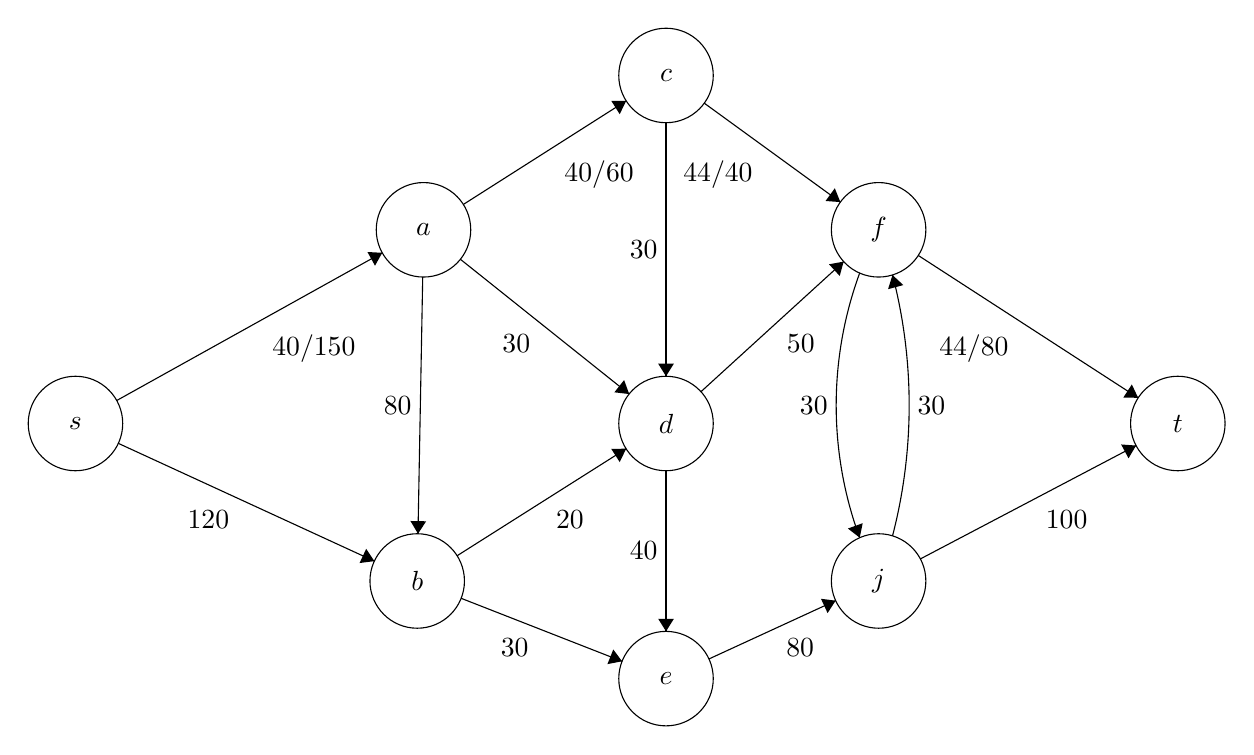
\begin{tikzpicture}[scale=0.2]
	\tikzstyle{every node}+=[inner sep=0pt]
	\draw [black] (4.3,-34.5) circle (3);
	\draw (4.3,-34.5) node {$s$};
	\draw [black] (41.8,-12.4) circle (3);
	\draw (41.8,-12.4) node {$c$};
	\draw [black] (26.4,-22.2) circle (3);
	\draw (26.4,-22.2) node {$a$};
	\draw [black] (26,-44.5) circle (3);
	\draw (26,-44.5) node {$b$};
	\draw [black] (41.8,-34.5) circle (3);
	\draw (41.8,-34.5) node {$d$};
	\draw [black] (41.8,-50.7) circle (3);
	\draw (41.8,-50.7) node {$e$};
	\draw [black] (55.3,-22.2) circle (3);
	\draw (55.3,-22.2) node {$f$};
	\draw [black] (55.3,-44.5) circle (3);
	\draw (55.3,-44.5) node {$j$};
	\draw [black] (74.3,-34.5) circle (3);
	\draw (74.3,-34.5) node {$t$};
	\draw [black] (6.92,-33.04) -- (23.78,-23.66);
	\fill [black] (23.78,-23.66) -- (22.84,-23.61) -- (23.32,-24.48);
	\draw (19.44,-28.86) node [below] {$40/150$};
	\draw [black] (7.02,-35.76) -- (23.28,-43.24);
	\fill [black] (23.28,-43.24) -- (22.76,-42.46) -- (22.34,-43.36);
	\draw (12.74,-40.02) node [below] {$120$};
	\draw [black] (26.35,-25.2) -- (26.05,-41.5);
	\fill [black] (26.05,-41.5) -- (26.57,-40.71) -- (25.57,-40.69);
	\draw (25.67,-33.35) node [left] {$80$};
	\draw [black] (28.93,-20.59) -- (39.27,-14.01);
	\fill [black] (39.27,-14.01) -- (38.33,-14.02) -- (38.86,-14.86);
	\draw (37.55,-17.8) node [below] {$40/60$};
	\draw [black] (28.74,-24.07) -- (39.46,-32.63);
	\fill [black] (39.46,-32.63) -- (39.14,-31.74) -- (38.52,-32.52);
	\draw (32.29,-28.84) node [below] {$30$};
	\draw [black] (28.53,-42.9) -- (39.27,-36.1);
	\fill [black] (39.27,-36.1) -- (38.32,-36.11) -- (38.86,-36.95);
	\draw (35.7,-40) node [below] {$20$};
	\draw [black] (28.79,-45.6) -- (39.01,-49.6);
	\fill [black] (39.01,-49.6) -- (38.45,-48.85) -- (38.08,-49.78);
	\draw (32.19,-48.13) node [below] {$30$};
	\draw [black] (41.8,-37.5) -- (41.8,-47.7);
	\fill [black] (41.8,-47.7) -- (42.3,-46.9) -- (41.3,-46.9);
	\draw (41.3,-42.6) node [left] {$40$};
	\draw [black] (41.8,-15.4) -- (41.8,-31.5);
	\fill [black] (41.8,-31.5) -- (42.3,-30.7) -- (41.3,-30.7);
	\draw (41.3,-23.45) node [left] {$30$};
	\draw [black] (44.53,-49.45) -- (52.57,-45.75);
	\fill [black] (52.57,-45.75) -- (51.64,-45.63) -- (52.06,-46.54);
	\draw (50.32,-48.11) node [below] {$80$};
	\draw [black] (44.02,-32.48) -- (53.08,-24.22);
	\fill [black] (53.08,-24.22) -- (52.15,-24.39) -- (52.83,-25.13);
	\draw (50.36,-28.84) node [below] {$50$};
	\draw [black] (54.097,-41.754) arc (-159.86286:-200.13714:24.411);
	\fill [black] (54.1,-41.75) -- (54.29,-40.83) -- (53.35,-41.17);
	\draw (52.1,-33.35) node [left] {$30$};
	\draw [black] (56.184,-25.066) arc (14.53791:-14.53791:33.002);
	\fill [black] (56.18,-25.07) -- (55.9,-25.97) -- (56.87,-25.71);
	\draw (57.74,-33.35) node [right] {$30$};
	\draw [black] (44.23,-14.16) -- (52.87,-20.44);
	\fill [black] (52.87,-20.44) -- (52.52,-19.56) -- (51.93,-20.37);
	\draw (45.1,-17.8) node [below] {$44/40$};
	\draw [black] (57.82,-23.83) -- (71.78,-32.87);
	\fill [black] (71.78,-32.87) -- (71.38,-32.02) -- (70.84,-32.85);
	\draw (61.35,-28.85) node [below] {$44/80$};
	\draw [black] (57.95,-43.1) -- (71.65,-35.9);
	\fill [black] (71.65,-35.9) -- (70.7,-35.83) -- (71.17,-36.71);
	\draw (67.24,-40.01) node [below] {$100$};
	\end{tikzpicture}
\end{center}

Path: $s \rightarrow a \rightarrow c \rightarrow f \rightarrow t$




\begin{center}
	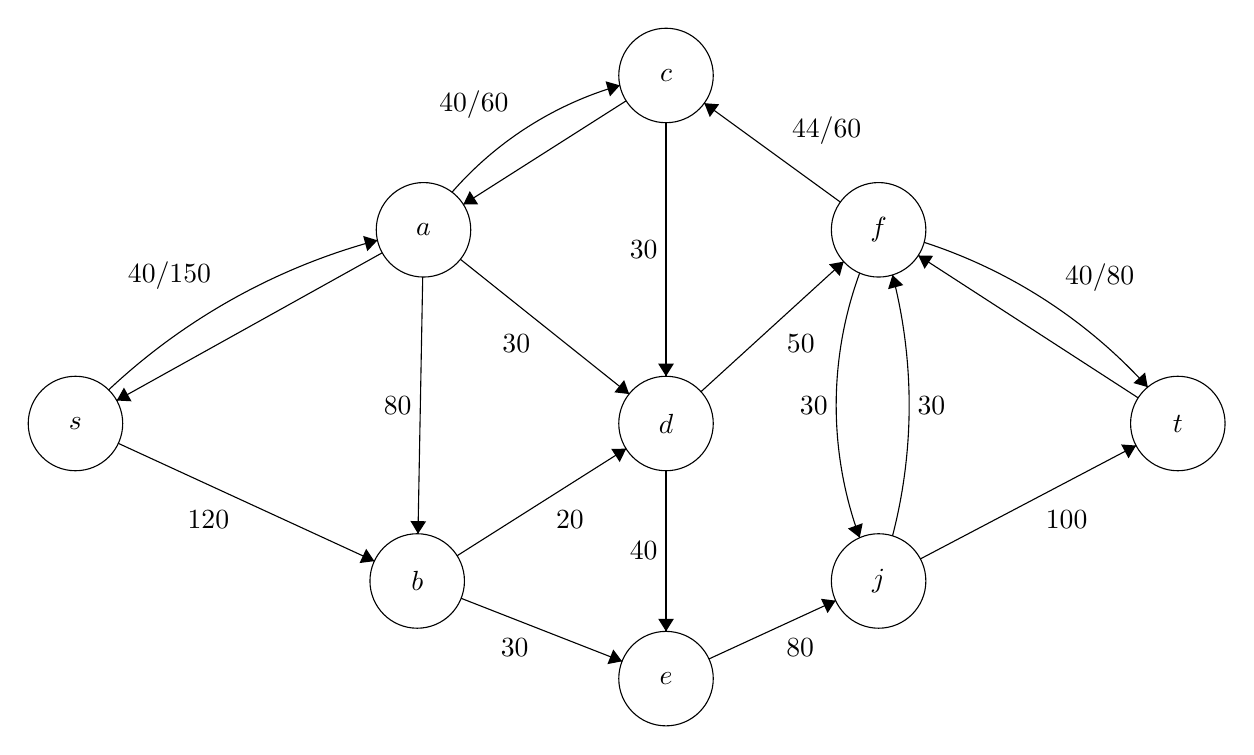
\begin{tikzpicture}[scale=0.2]
	\tikzstyle{every node}+=[inner sep=0pt]
	\draw [black] (4.3,-34.5) circle (3);
	\draw (4.3,-34.5) node {$s$};
	\draw [black] (41.8,-12.4) circle (3);
	\draw (41.8,-12.4) node {$c$};
	\draw [black] (26.4,-22.2) circle (3);
	\draw (26.4,-22.2) node {$a$};
	\draw [black] (26,-44.5) circle (3);
	\draw (26,-44.5) node {$b$};
	\draw [black] (41.8,-34.5) circle (3);
	\draw (41.8,-34.5) node {$d$};
	\draw [black] (41.8,-50.7) circle (3);
	\draw (41.8,-50.7) node {$e$};
	\draw [black] (55.3,-22.2) circle (3);
	\draw (55.3,-22.2) node {$f$};
	\draw [black] (55.3,-44.5) circle (3);
	\draw (55.3,-44.5) node {$j$};
	\draw [black] (74.3,-34.5) circle (3);
	\draw (74.3,-34.5) node {$t$};
	\draw [black] (6.407,-32.365) arc (133.2251:104.97212:40.018);
	\fill [black] (23.48,-22.87) -- (22.57,-22.59) -- (22.83,-23.56);
	\draw (10.27,-26.05) node [above] {$40/150$};
	\draw [black] (7.02,-35.76) -- (23.28,-43.24);
	\fill [black] (23.28,-43.24) -- (22.76,-42.46) -- (22.34,-43.36);
	\draw (12.74,-40.02) node [below] {$120$};
	\draw [black] (26.35,-25.2) -- (26.05,-41.5);
	\fill [black] (26.05,-41.5) -- (26.57,-40.71) -- (25.57,-40.69);
	\draw (25.67,-33.35) node [left] {$80$};
	\draw [black] (28.213,-19.812) arc (138.93683:106.00556:22.282);
	\fill [black] (38.87,-13.03) -- (37.96,-12.77) -- (38.24,-13.73);
	\draw (29.6,-15.15) node [above] {$40/60$};
	\draw [black] (28.74,-24.07) -- (39.46,-32.63);
	\fill [black] (39.46,-32.63) -- (39.14,-31.74) -- (38.52,-32.52);
	\draw (32.29,-28.84) node [below] {$30$};
	\draw [black] (28.79,-45.6) -- (39.01,-49.6);
	\fill [black] (39.01,-49.6) -- (38.45,-48.85) -- (38.08,-49.78);
	\draw (32.19,-48.13) node [below] {$30$};
	\draw [black] (41.8,-37.5) -- (41.8,-47.7);
	\fill [black] (41.8,-47.7) -- (42.3,-46.9) -- (41.3,-46.9);
	\draw (41.3,-42.6) node [left] {$40$};
	\draw [black] (41.8,-15.4) -- (41.8,-31.5);
	\fill [black] (41.8,-31.5) -- (42.3,-30.7) -- (41.3,-30.7);
	\draw (41.3,-23.45) node [left] {$30$};
	\draw [black] (44.53,-49.45) -- (52.57,-45.75);
	\fill [black] (52.57,-45.75) -- (51.64,-45.63) -- (52.06,-46.54);
	\draw (50.32,-48.11) node [below] {$80$};
	\draw [black] (44.02,-32.48) -- (53.08,-24.22);
	\fill [black] (53.08,-24.22) -- (52.15,-24.39) -- (52.83,-25.13);
	\draw (50.36,-28.84) node [below] {$50$};
	\draw [black] (54.097,-41.754) arc (-159.86286:-200.13714:24.411);
	\fill [black] (54.1,-41.75) -- (54.29,-40.83) -- (53.35,-41.17);
	\draw (52.1,-33.35) node [left] {$30$};
	\draw [black] (56.184,-25.066) arc (14.53791:-14.53791:33.002);
	\fill [black] (56.18,-25.07) -- (55.9,-25.97) -- (56.87,-25.71);
	\draw (57.74,-33.35) node [right] {$30$};
	\draw [black] (58.191,-22.996) arc (71.99098:42.17353:32.871);
	\fill [black] (72.39,-32.19) -- (72.22,-31.26) -- (71.48,-31.93);
	\draw (69.34,-26.16) node [above] {$40/80$};
	\draw [black] (57.95,-43.1) -- (71.65,-35.9);
	\fill [black] (71.65,-35.9) -- (70.7,-35.83) -- (71.17,-36.71);
	\draw (67.24,-40.01) node [below] {$100$};
	\draw [black] (23.78,-23.66) -- (6.92,-33.04);
	\fill [black] (6.92,-33.04) -- (7.86,-33.09) -- (7.38,-32.22);
	\draw [black] (39.27,-14.01) -- (28.93,-20.59);
	\fill [black] (28.93,-20.59) -- (29.87,-20.58) -- (29.34,-19.74);
	\draw [black] (52.87,-20.44) -- (44.23,-14.16);
	\fill [black] (44.23,-14.16) -- (44.58,-15.04) -- (45.17,-14.23);
	\draw (52,-16.8) node [above] {$44/60$};
	\draw [black] (71.78,-32.87) -- (57.82,-23.83);
	\fill [black] (57.82,-23.83) -- (58.22,-24.68) -- (58.76,-23.85);
	\draw [black] (28.53,-42.9) -- (39.27,-36.1);
	\fill [black] (39.27,-36.1) -- (38.32,-36.11) -- (38.86,-36.95);
	\draw (35.7,-40) node [below] {$20$};
	\end{tikzpicture}
\end{center}

Path: $s \rightarrow b \rightarrow e \rightarrow g \rightarrow t $



\begin{center}
	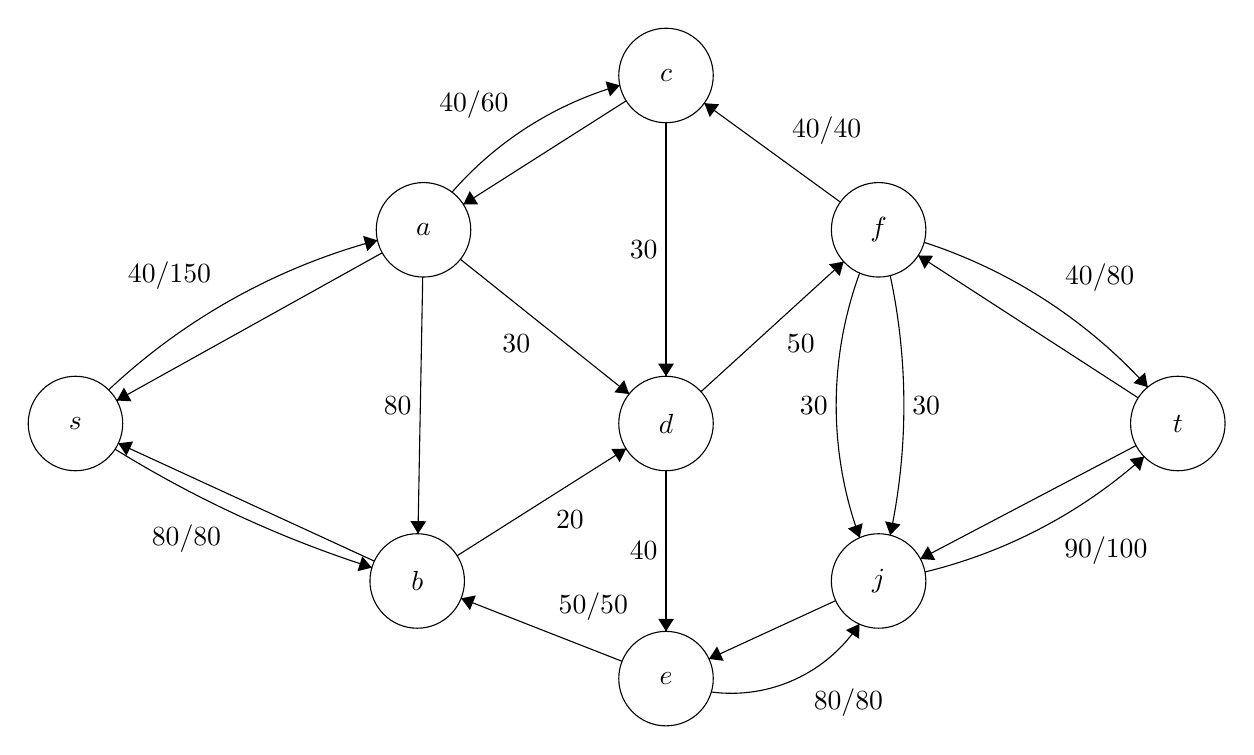
\begin{tikzpicture}[scale=0.2]
	\tikzstyle{every node}+=[inner sep=0pt]
	\draw [black] (4.3,-34.5) circle (3);
	\draw (4.3,-34.5) node {$s$};
	\draw [black] (41.8,-12.4) circle (3);
	\draw (41.8,-12.4) node {$c$};
	\draw [black] (26.4,-22.2) circle (3);
	\draw (26.4,-22.2) node {$a$};
	\draw [black] (26,-44.5) circle (3);
	\draw (26,-44.5) node {$b$};
	\draw [black] (41.8,-34.5) circle (3);
	\draw (41.8,-34.5) node {$d$};
	\draw [black] (41.8,-50.7) circle (3);
	\draw (41.8,-50.7) node {$e$};
	\draw [black] (55.3,-22.2) circle (3);
	\draw (55.3,-22.2) node {$f$};
	\draw [black] (55.3,-44.5) circle (3);
	\draw (55.3,-44.5) node {$j$};
	\draw [black] (74.3,-34.5) circle (3);
	\draw (74.3,-34.5) node {$t$};
	\draw [black] (6.407,-32.365) arc (133.2251:104.97212:40.018);
	\fill [black] (23.48,-22.87) -- (22.57,-22.59) -- (22.83,-23.56);
	\draw (10.27,-26.05) node [above] {$40/150$};
	\draw [black] (23.124,-43.646) arc (-107.71625:-121.76704:73.4);
	\fill [black] (23.12,-43.65) -- (22.51,-42.93) -- (22.21,-43.88);
	\draw (11.35,-40.92) node [below] {$80/80$};
	\draw [black] (26.35,-25.2) -- (26.05,-41.5);
	\fill [black] (26.05,-41.5) -- (26.57,-40.71) -- (25.57,-40.69);
	\draw (25.67,-33.35) node [left] {$80$};
	\draw [black] (28.213,-19.812) arc (138.93683:106.00556:22.282);
	\fill [black] (38.87,-13.03) -- (37.96,-12.77) -- (38.24,-13.73);
	\draw (29.6,-15.15) node [above] {$40/60$};
	\draw [black] (28.74,-24.07) -- (39.46,-32.63);
	\fill [black] (39.46,-32.63) -- (39.14,-31.74) -- (38.52,-32.52);
	\draw (32.29,-28.84) node [below] {$30$};
	\draw [black] (41.8,-37.5) -- (41.8,-47.7);
	\fill [black] (41.8,-47.7) -- (42.3,-46.9) -- (41.3,-46.9);
	\draw (41.3,-42.6) node [left] {$40$};
	\draw [black] (41.8,-15.4) -- (41.8,-31.5);
	\fill [black] (41.8,-31.5) -- (42.3,-30.7) -- (41.3,-30.7);
	\draw (41.3,-23.45) node [left] {$30$};
	\draw [black] (54.076,-47.226) arc (-33.04242:-97.62279:9.693);
	\fill [black] (54.08,-47.23) -- (53.22,-47.62) -- (54.06,-48.17);
	\draw (53.38,-51.28) node [below] {$80/80$};
	\draw [black] (44.02,-32.48) -- (53.08,-24.22);
	\fill [black] (53.08,-24.22) -- (52.15,-24.39) -- (52.83,-25.13);
	\draw (50.36,-28.84) node [below] {$50$};
	\draw [black] (54.097,-41.754) arc (-159.86286:-200.13714:24.411);
	\fill [black] (54.1,-41.75) -- (54.29,-40.83) -- (53.35,-41.17);
	\draw (52.1,-33.35) node [left] {$30$};
	\draw [black] (58.191,-22.996) arc (71.99098:42.17353:32.871);
	\fill [black] (72.39,-32.19) -- (72.22,-31.26) -- (71.48,-31.93);
	\draw (69.34,-26.16) node [above] {$40/80$};
	\draw [black] (72.162,-36.603) arc (-48.13704:-76.34588:32.271);
	\fill [black] (72.16,-36.6) -- (71.23,-36.76) -- (71.9,-37.51);
	\draw (69.73,-41.64) node [below] {$90/100$};
	\draw [black] (23.78,-23.66) -- (6.92,-33.04);
	\fill [black] (6.92,-33.04) -- (7.86,-33.09) -- (7.38,-32.22);
	\draw [black] (39.27,-14.01) -- (28.93,-20.59);
	\fill [black] (28.93,-20.59) -- (29.87,-20.58) -- (29.34,-19.74);
	\draw [black] (52.87,-20.44) -- (44.23,-14.16);
	\fill [black] (44.23,-14.16) -- (44.58,-15.04) -- (45.17,-14.23);
	\draw (52,-16.8) node [above] {$40/40$};
	\draw [black] (71.78,-32.87) -- (57.82,-23.83);
	\fill [black] (57.82,-23.83) -- (58.22,-24.68) -- (58.76,-23.85);
	\draw [black] (28.53,-42.9) -- (39.27,-36.1);
	\fill [black] (39.27,-36.1) -- (38.32,-36.11) -- (38.86,-36.95);
	\draw (35.7,-40) node [below] {$20$};
	\draw [black] (39.01,-49.6) -- (28.79,-45.6);
	\fill [black] (28.79,-45.6) -- (29.35,-46.35) -- (29.72,-45.42);
	\draw (37.18,-47.03) node [above] {$50/50$};
	\draw [black] (52.57,-45.75) -- (44.53,-49.45);
	\fill [black] (44.53,-49.45) -- (45.46,-49.57) -- (45.04,-48.66);
	\draw [black] (71.65,-35.9) -- (57.95,-43.1);
	\fill [black] (57.95,-43.1) -- (58.9,-43.17) -- (58.43,-42.29);
	\draw [black] (56.036,-25.107) arc (12.03704:-12.03704:39.524);
	\fill [black] (56.04,-41.59) -- (56.69,-40.91) -- (55.71,-40.71);
	\draw (57.41,-33.35) node [right] {$30$};
	\draw [black] (23.28,-43.24) -- (7.02,-35.76);
	\fill [black] (7.02,-35.76) -- (7.54,-36.54) -- (7.96,-35.64);
	\end{tikzpicture}
\end{center}


Path: $s \leftrightarrow a \leftrightarrow c \rightarrow d \rightarrow f \rightarrow t$



\begin{center}
	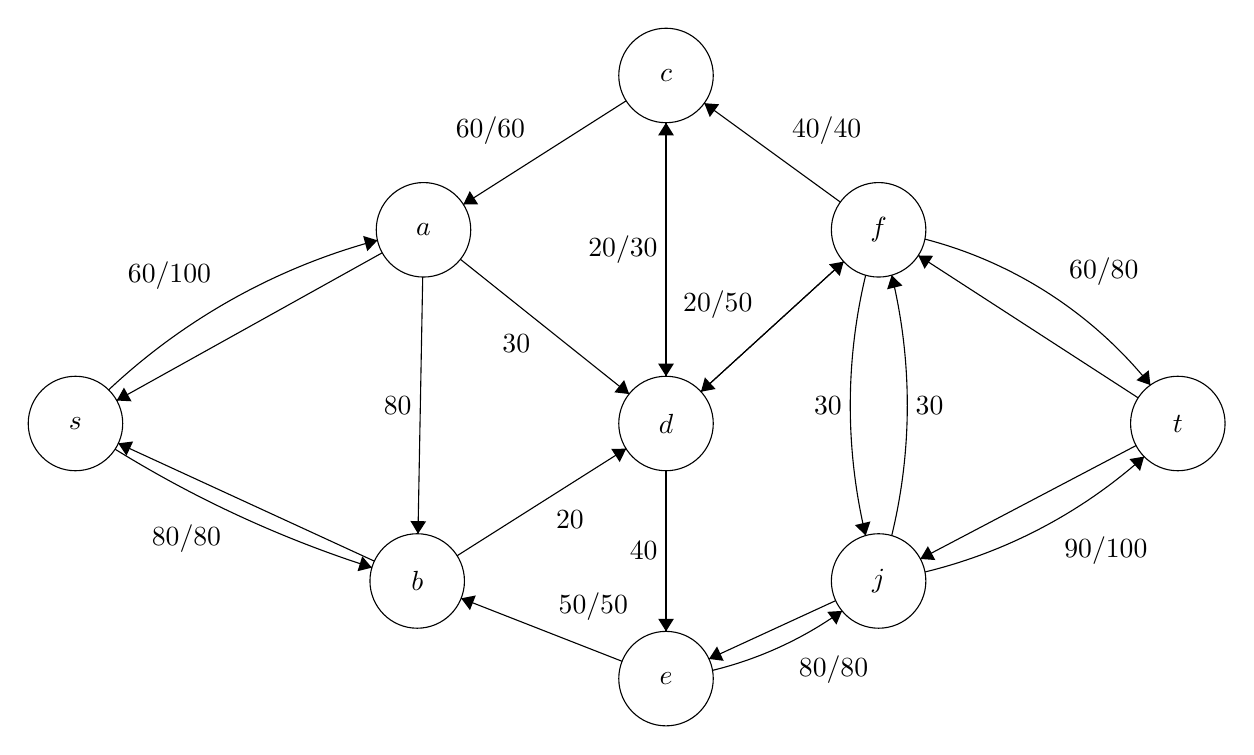
\begin{tikzpicture}[scale=0.2]
	\tikzstyle{every node}+=[inner sep=0pt]
	\draw [black] (4.3,-34.5) circle (3);
	\draw (4.3,-34.5) node {$s$};
	\draw [black] (41.8,-12.4) circle (3);
	\draw (41.8,-12.4) node {$c$};
	\draw [black] (26.4,-22.2) circle (3);
	\draw (26.4,-22.2) node {$a$};
	\draw [black] (26,-44.5) circle (3);
	\draw (26,-44.5) node {$b$};
	\draw [black] (41.8,-34.5) circle (3);
	\draw (41.8,-34.5) node {$d$};
	\draw [black] (41.8,-50.7) circle (3);
	\draw (41.8,-50.7) node {$e$};
	\draw [black] (55.3,-22.2) circle (3);
	\draw (55.3,-22.2) node {$f$};
	\draw [black] (55.3,-44.5) circle (3);
	\draw (55.3,-44.5) node {$j$};
	\draw [black] (74.3,-34.5) circle (3);
	\draw (74.3,-34.5) node {$t$};
	\draw [black] (6.407,-32.365) arc (133.2251:104.97212:40.018);
	\fill [black] (23.48,-22.87) -- (22.57,-22.59) -- (22.83,-23.56);
	\draw (10.27,-26.05) node [above] {$60/100$};
	\draw [black] (23.124,-43.646) arc (-107.71625:-121.76704:73.4);
	\fill [black] (23.12,-43.65) -- (22.51,-42.93) -- (22.21,-43.88);
	\draw (11.35,-40.92) node [below] {$80/80$};
	\draw [black] (26.35,-25.2) -- (26.05,-41.5);
	\fill [black] (26.05,-41.5) -- (26.57,-40.71) -- (25.57,-40.69);
	\draw (25.67,-33.35) node [left] {$80$};
	\draw [black] (28.74,-24.07) -- (39.46,-32.63);
	\fill [black] (39.46,-32.63) -- (39.14,-31.74) -- (38.52,-32.52);
	\draw (32.29,-28.84) node [below] {$30$};
	\draw [black] (41.8,-37.5) -- (41.8,-47.7);
	\fill [black] (41.8,-47.7) -- (42.3,-46.9) -- (41.3,-46.9);
	\draw (41.3,-42.6) node [left] {$40$};
	\draw [black] (41.8,-15.4) -- (41.8,-31.5);
	\fill [black] (41.8,-31.5) -- (42.3,-30.7) -- (41.3,-30.7);
	\draw (41.3,-23.45) node [left] {$20/30$};
	\draw [black] (52.979,-46.398) arc (-54.34063:-76.32459:23.741);
	\fill [black] (52.98,-46.4) -- (52.04,-46.46) -- (52.62,-47.27);
	\draw (52.44,-49.21) node [below] {$80/80$};
	\draw [black] (44.02,-32.48) -- (53.08,-24.22);
	\fill [black] (53.08,-24.22) -- (52.15,-24.39) -- (52.83,-25.13);
	\draw (45.09,-27.86) node [above] {$20/50$};
	\draw [black] (54.477,-41.616) arc (-166.50769:-193.49231:35.428);
	\fill [black] (54.48,-41.62) -- (54.78,-40.72) -- (53.8,-40.95);
	\draw (53,-33.35) node [left] {$30$};
	\draw [black] (58.24,-22.791) arc (75.45217:38.71234:27.06);
	\fill [black] (72.56,-32.06) -- (72.45,-31.12) -- (71.67,-31.75);
	\draw (69.6,-25.77) node [above] {$60/80$};
	\draw [black] (72.162,-36.603) arc (-48.13704:-76.34588:32.271);
	\fill [black] (72.16,-36.6) -- (71.23,-36.76) -- (71.9,-37.51);
	\draw (69.73,-41.64) node [below] {$90/100$};
	\draw [black] (23.78,-23.66) -- (6.92,-33.04);
	\fill [black] (6.92,-33.04) -- (7.86,-33.09) -- (7.38,-32.22);
	\draw [black] (39.27,-14.01) -- (28.93,-20.59);
	\fill [black] (28.93,-20.59) -- (29.87,-20.58) -- (29.34,-19.74);
	\draw (30.65,-16.8) node [above] {$60/60$};
	\draw [black] (52.87,-20.44) -- (44.23,-14.16);
	\fill [black] (44.23,-14.16) -- (44.58,-15.04) -- (45.17,-14.23);
	\draw (52,-16.8) node [above] {$40/40$};
	\draw [black] (71.78,-32.87) -- (57.82,-23.83);
	\fill [black] (57.82,-23.83) -- (58.22,-24.68) -- (58.76,-23.85);
	\draw [black] (28.53,-42.9) -- (39.27,-36.1);
	\fill [black] (39.27,-36.1) -- (38.32,-36.11) -- (38.86,-36.95);
	\draw (35.7,-40) node [below] {$20$};
	\draw [black] (39.01,-49.6) -- (28.79,-45.6);
	\fill [black] (28.79,-45.6) -- (29.35,-46.35) -- (29.72,-45.42);
	\draw (37.18,-47.03) node [above] {$50/50$};
	\draw [black] (52.57,-45.75) -- (44.53,-49.45);
	\fill [black] (44.53,-49.45) -- (45.46,-49.57) -- (45.04,-48.66);
	\draw [black] (71.65,-35.9) -- (57.95,-43.1);
	\fill [black] (57.95,-43.1) -- (58.9,-43.17) -- (58.43,-42.29);
	\draw [black] (23.28,-43.24) -- (7.02,-35.76);
	\fill [black] (7.02,-35.76) -- (7.54,-36.54) -- (7.96,-35.64);
	\draw [black] (41.8,-31.5) -- (41.8,-15.4);
	\fill [black] (41.8,-15.4) -- (41.3,-16.2) -- (42.3,-16.2);
	\draw [black] (53.08,-24.22) -- (44.02,-32.48);
	\fill [black] (44.02,-32.48) -- (44.95,-32.31) -- (44.27,-31.57);
	\draw [black] (56.132,-25.081) arc (13.65635:-13.65635:35.022);
	\fill [black] (56.13,-25.08) -- (55.84,-25.98) -- (56.81,-25.74);
	\draw (57.62,-33.35) node [right] {$30$};
	\end{tikzpicture}
\end{center}


Path: $s \leftrightarrow b \rightarrow d \rightarrow e \leftrightarrow g \leftrightarrow t$



\begin{center}
	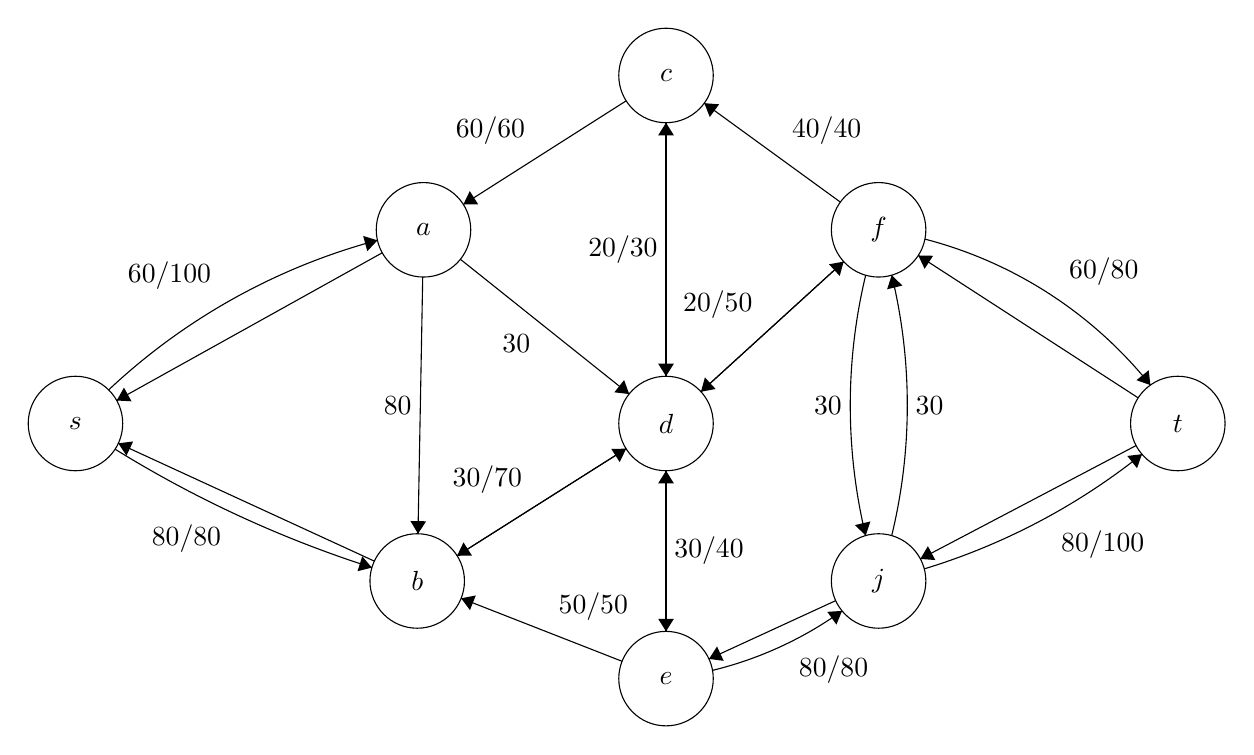
\begin{tikzpicture}[scale=0.2]
	\tikzstyle{every node}+=[inner sep=0pt]
	\draw [black] (4.3,-34.5) circle (3);
	\draw (4.3,-34.5) node {$s$};
	\draw [black] (41.8,-12.4) circle (3);
	\draw (41.8,-12.4) node {$c$};
	\draw [black] (26.4,-22.2) circle (3);
	\draw (26.4,-22.2) node {$a$};
	\draw [black] (26,-44.5) circle (3);
	\draw (26,-44.5) node {$b$};
	\draw [black] (41.8,-34.5) circle (3);
	\draw (41.8,-34.5) node {$d$};
	\draw [black] (41.8,-50.7) circle (3);
	\draw (41.8,-50.7) node {$e$};
	\draw [black] (55.3,-22.2) circle (3);
	\draw (55.3,-22.2) node {$f$};
	\draw [black] (55.3,-44.5) circle (3);
	\draw (55.3,-44.5) node {$j$};
	\draw [black] (74.3,-34.5) circle (3);
	\draw (74.3,-34.5) node {$t$};
	\draw [black] (6.407,-32.365) arc (133.2251:104.97212:40.018);
	\fill [black] (23.48,-22.87) -- (22.57,-22.59) -- (22.83,-23.56);
	\draw (10.27,-26.05) node [above] {$60/100$};
	\draw [black] (23.124,-43.646) arc (-107.71625:-121.76704:73.4);
	\fill [black] (23.12,-43.65) -- (22.51,-42.93) -- (22.21,-43.88);
	\draw (11.35,-40.92) node [below] {$80/80$};
	\draw [black] (26.35,-25.2) -- (26.05,-41.5);
	\fill [black] (26.05,-41.5) -- (26.57,-40.71) -- (25.57,-40.69);
	\draw (25.67,-33.35) node [left] {$80$};
	\draw [black] (28.74,-24.07) -- (39.46,-32.63);
	\fill [black] (39.46,-32.63) -- (39.14,-31.74) -- (38.52,-32.52);
	\draw (32.29,-28.84) node [below] {$30$};
	\draw [black] (41.8,-37.5) -- (41.8,-47.7);
	\fill [black] (41.8,-47.7) -- (42.3,-46.9) -- (41.3,-46.9);
	\draw (42.3,-42.6) node [right] {$30/40$};
	\draw [black] (41.8,-15.4) -- (41.8,-31.5);
	\fill [black] (41.8,-31.5) -- (42.3,-30.7) -- (41.3,-30.7);
	\draw (41.3,-23.45) node [left] {$20/30$};
	\draw [black] (52.979,-46.398) arc (-54.34063:-76.32459:23.741);
	\fill [black] (52.98,-46.4) -- (52.04,-46.46) -- (52.62,-47.27);
	\draw (52.44,-49.21) node [below] {$80/80$};
	\draw [black] (44.02,-32.48) -- (53.08,-24.22);
	\fill [black] (53.08,-24.22) -- (52.15,-24.39) -- (52.83,-25.13);
	\draw (45.09,-27.86) node [above] {$20/50$};
	\draw [black] (54.477,-41.616) arc (-166.50769:-193.49231:35.428);
	\fill [black] (54.48,-41.62) -- (54.78,-40.72) -- (53.8,-40.95);
	\draw (53,-33.35) node [left] {$30$};
	\draw [black] (58.24,-22.791) arc (75.45217:38.71234:27.06);
	\fill [black] (72.56,-32.06) -- (72.45,-31.12) -- (71.67,-31.75);
	\draw (69.6,-25.77) node [above] {$60/80$};
	\draw [black] (72.024,-36.454) arc (-51.42398:-73.05894:41.622);
	\fill [black] (72.02,-36.45) -- (71.09,-36.56) -- (71.71,-37.34);
	\draw (69.53,-41.26) node [below] {$80/100$};
	\draw [black] (23.78,-23.66) -- (6.92,-33.04);
	\fill [black] (6.92,-33.04) -- (7.86,-33.09) -- (7.38,-32.22);
	\draw [black] (39.27,-14.01) -- (28.93,-20.59);
	\fill [black] (28.93,-20.59) -- (29.87,-20.58) -- (29.34,-19.74);
	\draw (30.65,-16.8) node [above] {$60/60$};
	\draw [black] (52.87,-20.44) -- (44.23,-14.16);
	\fill [black] (44.23,-14.16) -- (44.58,-15.04) -- (45.17,-14.23);
	\draw (52,-16.8) node [above] {$40/40$};
	\draw [black] (71.78,-32.87) -- (57.82,-23.83);
	\fill [black] (57.82,-23.83) -- (58.22,-24.68) -- (58.76,-23.85);
	\draw [black] (28.53,-42.9) -- (39.27,-36.1);
	\fill [black] (39.27,-36.1) -- (38.32,-36.11) -- (38.86,-36.95);
	\draw (30.45,-39) node [above] {$30/70$};
	\draw [black] (39.01,-49.6) -- (28.79,-45.6);
	\fill [black] (28.79,-45.6) -- (29.35,-46.35) -- (29.72,-45.42);
	\draw (37.18,-47.03) node [above] {$50/50$};
	\draw [black] (52.57,-45.75) -- (44.53,-49.45);
	\fill [black] (44.53,-49.45) -- (45.46,-49.57) -- (45.04,-48.66);
	\draw [black] (71.65,-35.9) -- (57.95,-43.1);
	\fill [black] (57.95,-43.1) -- (58.9,-43.17) -- (58.43,-42.29);
	\draw [black] (23.28,-43.24) -- (7.02,-35.76);
	\fill [black] (7.02,-35.76) -- (7.54,-36.54) -- (7.96,-35.64);
	\draw [black] (41.8,-31.5) -- (41.8,-15.4);
	\fill [black] (41.8,-15.4) -- (41.3,-16.2) -- (42.3,-16.2);
	\draw [black] (53.08,-24.22) -- (44.02,-32.48);
	\fill [black] (44.02,-32.48) -- (44.95,-32.31) -- (44.27,-31.57);
	\draw [black] (56.132,-25.081) arc (13.65635:-13.65635:35.022);
	\fill [black] (56.13,-25.08) -- (55.84,-25.98) -- (56.81,-25.74);
	\draw (57.62,-33.35) node [right] {$30$};
	\draw [black] (39.27,-36.1) -- (28.53,-42.9);
	\fill [black] (28.53,-42.9) -- (29.48,-42.89) -- (28.94,-42.05);
	\draw [black] (41.8,-47.7) -- (41.8,-37.5);
	\fill [black] (41.8,-37.5) -- (41.3,-38.3) -- (42.3,-38.3);
	\end{tikzpicture}
\end{center}


Path: $s \leftrightarrow b \leftrightarrow d \leftrightarrow f \leftrightarrow t$







	
	\begin{center}
		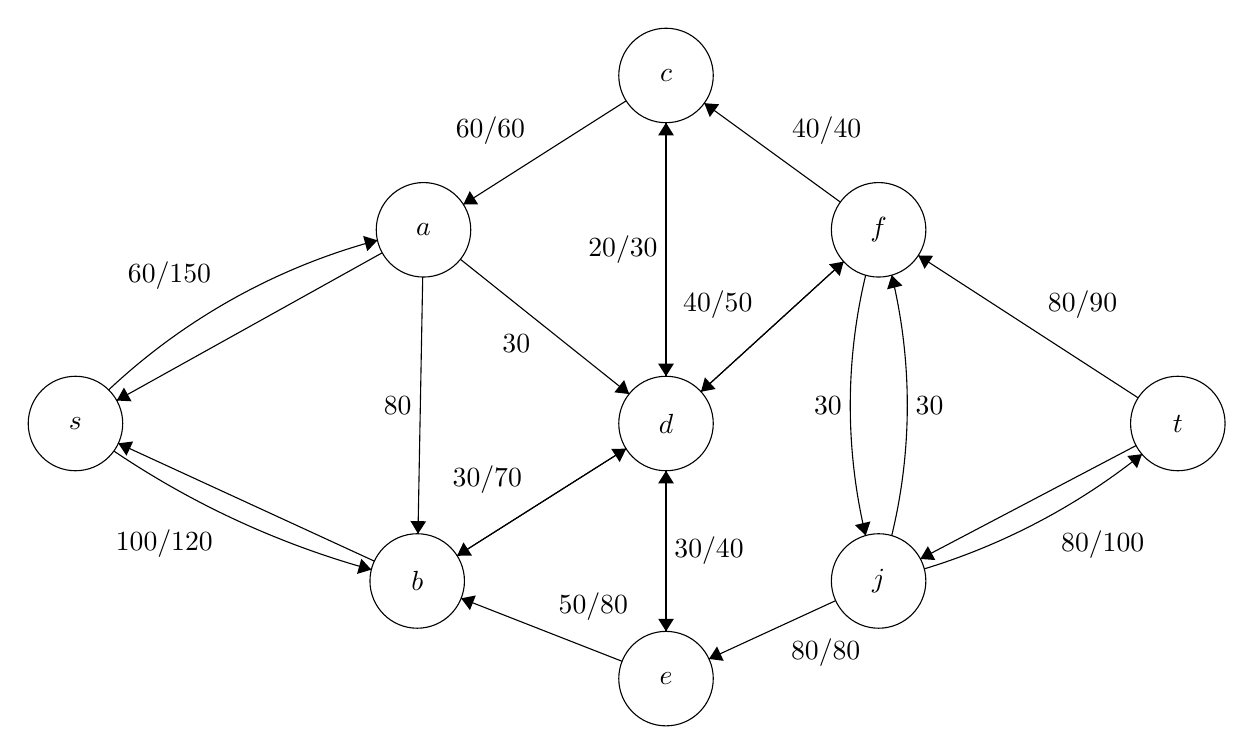
\begin{tikzpicture}[scale=0.2]
		\tikzstyle{every node}+=[inner sep=0pt]
		\draw [black] (4.3,-34.5) circle (3);
		\draw (4.3,-34.5) node {$s$};
		\draw [black] (41.8,-12.4) circle (3);
		\draw (41.8,-12.4) node {$c$};
		\draw [black] (26.4,-22.2) circle (3);
		\draw (26.4,-22.2) node {$a$};
		\draw [black] (26,-44.5) circle (3);
		\draw (26,-44.5) node {$b$};
		\draw [black] (41.8,-34.5) circle (3);
		\draw (41.8,-34.5) node {$d$};
		\draw [black] (41.8,-50.7) circle (3);
		\draw (41.8,-50.7) node {$e$};
		\draw [black] (55.3,-22.2) circle (3);
		\draw (55.3,-22.2) node {$f$};
		\draw [black] (55.3,-44.5) circle (3);
		\draw (55.3,-44.5) node {$j$};
		\draw [black] (74.3,-34.5) circle (3);
		\draw (74.3,-34.5) node {$t$};
		\draw [black] (6.407,-32.365) arc (133.2251:104.97212:40.018);
		\fill [black] (23.48,-22.87) -- (22.57,-22.59) -- (22.83,-23.56);
		\draw (10.27,-26.05) node [above] {$60/150$};
		\draw [black] (23.088,-43.78) arc (-105.42481:-124.05847:55.597);
		\fill [black] (23.09,-43.78) -- (22.45,-43.09) -- (22.18,-44.05);
		\draw (9.94,-41.22) node [below] {$100/120$};
		\draw [black] (26.35,-25.2) -- (26.05,-41.5);
		\fill [black] (26.05,-41.5) -- (26.57,-40.71) -- (25.57,-40.69);
		\draw (25.67,-33.35) node [left] {$80$};
		\draw [black] (28.74,-24.07) -- (39.46,-32.63);
		\fill [black] (39.46,-32.63) -- (39.14,-31.74) -- (38.52,-32.52);
		\draw (32.29,-28.84) node [below] {$30$};
		\draw [black] (41.8,-37.5) -- (41.8,-47.7);
		\fill [black] (41.8,-47.7) -- (42.3,-46.9) -- (41.3,-46.9);
		\draw (42.3,-42.6) node [right] {$30/40$};
		\draw [black] (41.8,-15.4) -- (41.8,-31.5);
		\fill [black] (41.8,-31.5) -- (42.3,-30.7) -- (41.3,-30.7);
		\draw (41.3,-23.45) node [left] {$20/30$};
		\draw [black] (44.02,-32.48) -- (53.08,-24.22);
		\fill [black] (53.08,-24.22) -- (52.15,-24.39) -- (52.83,-25.13);
		\draw (45.09,-27.86) node [above] {$40/50$};
		\draw [black] (54.477,-41.616) arc (-166.50769:-193.49231:35.428);
		\fill [black] (54.48,-41.62) -- (54.78,-40.72) -- (53.8,-40.95);
		\draw (53,-33.35) node [left] {$30$};
		\draw [black] (72.024,-36.454) arc (-51.42398:-73.05894:41.622);
		\fill [black] (72.02,-36.45) -- (71.09,-36.56) -- (71.71,-37.34);
		\draw (69.53,-41.26) node [below] {$80/100$};
		\draw [black] (23.78,-23.66) -- (6.92,-33.04);
		\fill [black] (6.92,-33.04) -- (7.86,-33.09) -- (7.38,-32.22);
		\draw [black] (39.27,-14.01) -- (28.93,-20.59);
		\fill [black] (28.93,-20.59) -- (29.87,-20.58) -- (29.34,-19.74);
		\draw (30.65,-16.8) node [above] {$60/60$};
		\draw [black] (52.87,-20.44) -- (44.23,-14.16);
		\fill [black] (44.23,-14.16) -- (44.58,-15.04) -- (45.17,-14.23);
		\draw (52,-16.8) node [above] {$40/40$};
		\draw [black] (71.78,-32.87) -- (57.82,-23.83);
		\fill [black] (57.82,-23.83) -- (58.22,-24.68) -- (58.76,-23.85);
		\draw (68.25,-27.85) node [above] {$80/90$};
		\draw [black] (28.53,-42.9) -- (39.27,-36.1);
		\fill [black] (39.27,-36.1) -- (38.32,-36.11) -- (38.86,-36.95);
		\draw (30.45,-39) node [above] {$30/70$};
		\draw [black] (39.01,-49.6) -- (28.79,-45.6);
		\fill [black] (28.79,-45.6) -- (29.35,-46.35) -- (29.72,-45.42);
		\draw (37.18,-47.03) node [above] {$50/80$};
		\draw [black] (52.57,-45.75) -- (44.53,-49.45);
		\fill [black] (44.53,-49.45) -- (45.46,-49.57) -- (45.04,-48.66);
		\draw (51.94,-48.13) node [below] {$80/80$};
		\draw [black] (71.65,-35.9) -- (57.95,-43.1);
		\fill [black] (57.95,-43.1) -- (58.9,-43.17) -- (58.43,-42.29);
		\draw [black] (23.28,-43.24) -- (7.02,-35.76);
		\fill [black] (7.02,-35.76) -- (7.54,-36.54) -- (7.96,-35.64);
		\draw [black] (41.8,-31.5) -- (41.8,-15.4);
		\fill [black] (41.8,-15.4) -- (41.3,-16.2) -- (42.3,-16.2);
		\draw [black] (53.08,-24.22) -- (44.02,-32.48);
		\fill [black] (44.02,-32.48) -- (44.95,-32.31) -- (44.27,-31.57);
		\draw [black] (56.132,-25.081) arc (13.65635:-13.65635:35.022);
		\fill [black] (56.13,-25.08) -- (55.84,-25.98) -- (56.81,-25.74);
		\draw (57.62,-33.35) node [right] {$30$};
		\draw [black] (39.27,-36.1) -- (28.53,-42.9);
		\fill [black] (28.53,-42.9) -- (29.48,-42.89) -- (28.94,-42.05);
		\draw [black] (41.8,-47.7) -- (41.8,-37.5);
		\fill [black] (41.8,-37.5) -- (41.3,-38.3) -- (42.3,-38.3);
		\end{tikzpicture}
	\end{center}


Path: $s \leftrightarrow a \rightarrow d \leftrightarrow f \leftarrow g \leftrightarrow t$



\begin{center}
	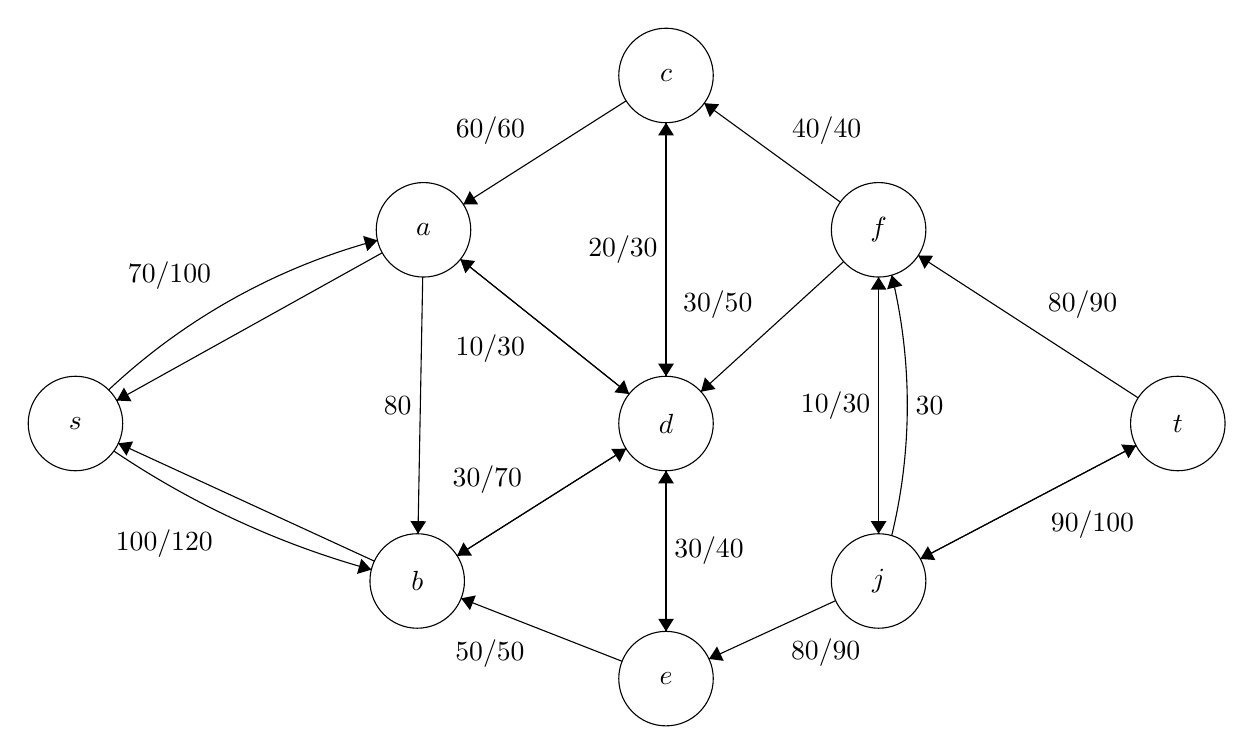
\begin{tikzpicture}[scale=0.2]
	\tikzstyle{every node}+=[inner sep=0pt]
	\draw [black] (4.3,-34.5) circle (3);
	\draw (4.3,-34.5) node {$s$};
	\draw [black] (41.8,-12.4) circle (3);
	\draw (41.8,-12.4) node {$c$};
	\draw [black] (26.4,-22.2) circle (3);
	\draw (26.4,-22.2) node {$a$};
	\draw [black] (26,-44.5) circle (3);
	\draw (26,-44.5) node {$b$};
	\draw [black] (41.8,-34.5) circle (3);
	\draw (41.8,-34.5) node {$d$};
	\draw [black] (41.8,-50.7) circle (3);
	\draw (41.8,-50.7) node {$e$};
	\draw [black] (55.3,-22.2) circle (3);
	\draw (55.3,-22.2) node {$f$};
	\draw [black] (55.3,-44.5) circle (3);
	\draw (55.3,-44.5) node {$j$};
	\draw [black] (74.3,-34.5) circle (3);
	\draw (74.3,-34.5) node {$t$};
	\draw [black] (6.407,-32.365) arc (133.2251:104.97212:40.018);
	\fill [black] (23.48,-22.87) -- (22.57,-22.59) -- (22.83,-23.56);
	\draw (10.27,-26.05) node [above] {$70/100$};
	\draw [black] (23.088,-43.78) arc (-105.42481:-124.05847:55.597);
	\fill [black] (23.09,-43.78) -- (22.45,-43.09) -- (22.18,-44.05);
	\draw (9.94,-41.22) node [below] {$100/120$};
	\draw [black] (26.35,-25.2) -- (26.05,-41.5);
	\fill [black] (26.05,-41.5) -- (26.57,-40.71) -- (25.57,-40.69);
	\draw (25.67,-33.35) node [left] {$80$};
	\draw [black] (28.74,-24.07) -- (39.46,-32.63);
	\fill [black] (39.46,-32.63) -- (39.14,-31.74) -- (38.52,-32.52);
	\draw (30.64,-28.84) node [below] {$10/30$};
	\draw [black] (41.8,-37.5) -- (41.8,-47.7);
	\fill [black] (41.8,-47.7) -- (42.3,-46.9) -- (41.3,-46.9);
	\draw (42.3,-42.6) node [right] {$30/40$};
	\draw [black] (41.8,-15.4) -- (41.8,-31.5);
	\fill [black] (41.8,-31.5) -- (42.3,-30.7) -- (41.3,-30.7);
	\draw (41.3,-23.45) node [left] {$20/30$};
	\draw [black] (55.3,-25.2) -- (55.3,-41.5);
	\fill [black] (55.3,-41.5) -- (55.8,-40.7) -- (54.8,-40.7);
	\draw (54.8,-33.35) node [left] {$10/30$};
	\draw [black] (57.95,-43.1) -- (71.65,-35.9);
	\fill [black] (71.65,-35.9) -- (70.7,-35.83) -- (71.17,-36.71);
	\draw (68.88,-40.01) node [below] {$90/100$};
	\draw [black] (23.78,-23.66) -- (6.92,-33.04);
	\fill [black] (6.92,-33.04) -- (7.86,-33.09) -- (7.38,-32.22);
	\draw [black] (39.27,-14.01) -- (28.93,-20.59);
	\fill [black] (28.93,-20.59) -- (29.87,-20.58) -- (29.34,-19.74);
	\draw (30.65,-16.8) node [above] {$60/60$};
	\draw [black] (52.87,-20.44) -- (44.23,-14.16);
	\fill [black] (44.23,-14.16) -- (44.58,-15.04) -- (45.17,-14.23);
	\draw (52,-16.8) node [above] {$40/40$};
	\draw [black] (71.78,-32.87) -- (57.82,-23.83);
	\fill [black] (57.82,-23.83) -- (58.22,-24.68) -- (58.76,-23.85);
	\draw (68.25,-27.85) node [above] {$80/90$};
	\draw [black] (28.53,-42.9) -- (39.27,-36.1);
	\fill [black] (39.27,-36.1) -- (38.32,-36.11) -- (38.86,-36.95);
	\draw (30.45,-39) node [above] {$30/70$};
	\draw [black] (39.01,-49.6) -- (28.79,-45.6);
	\fill [black] (28.79,-45.6) -- (29.35,-46.35) -- (29.72,-45.42);
	\draw (30.62,-48.17) node [below] {$50/50$};
	\draw [black] (52.57,-45.75) -- (44.53,-49.45);
	\fill [black] (44.53,-49.45) -- (45.46,-49.57) -- (45.04,-48.66);
	\draw (51.94,-48.13) node [below] {$80/90$};
	\draw [black] (71.65,-35.9) -- (57.95,-43.1);
	\fill [black] (57.95,-43.1) -- (58.9,-43.17) -- (58.43,-42.29);
	\draw [black] (23.28,-43.24) -- (7.02,-35.76);
	\fill [black] (7.02,-35.76) -- (7.54,-36.54) -- (7.96,-35.64);
	\draw [black] (41.8,-31.5) -- (41.8,-15.4);
	\fill [black] (41.8,-15.4) -- (41.3,-16.2) -- (42.3,-16.2);
	\draw [black] (53.08,-24.22) -- (44.02,-32.48);
	\fill [black] (44.02,-32.48) -- (44.95,-32.31) -- (44.27,-31.57);
	\draw (45.09,-27.86) node [above] {$30/50$};
	\draw [black] (56.132,-25.081) arc (13.65635:-13.65635:35.022);
	\fill [black] (56.13,-25.08) -- (55.84,-25.98) -- (56.81,-25.74);
	\draw (57.62,-33.35) node [right] {$30$};
	\draw [black] (39.27,-36.1) -- (28.53,-42.9);
	\fill [black] (28.53,-42.9) -- (29.48,-42.89) -- (28.94,-42.05);
	\draw [black] (41.8,-47.7) -- (41.8,-37.5);
	\fill [black] (41.8,-37.5) -- (41.3,-38.3) -- (42.3,-38.3);
	\draw [black] (39.46,-32.63) -- (28.74,-24.07);
	\fill [black] (28.74,-24.07) -- (29.06,-24.96) -- (29.68,-24.18);
	\draw [black] (55.3,-41.5) -- (55.3,-25.2);
	\fill [black] (55.3,-25.2) -- (54.8,-26) -- (55.8,-26);
	\end{tikzpicture}
\end{center}

Path: no available path $s \rightarrow t$.
\\\\
Resulting Graph:
\begin{center}
	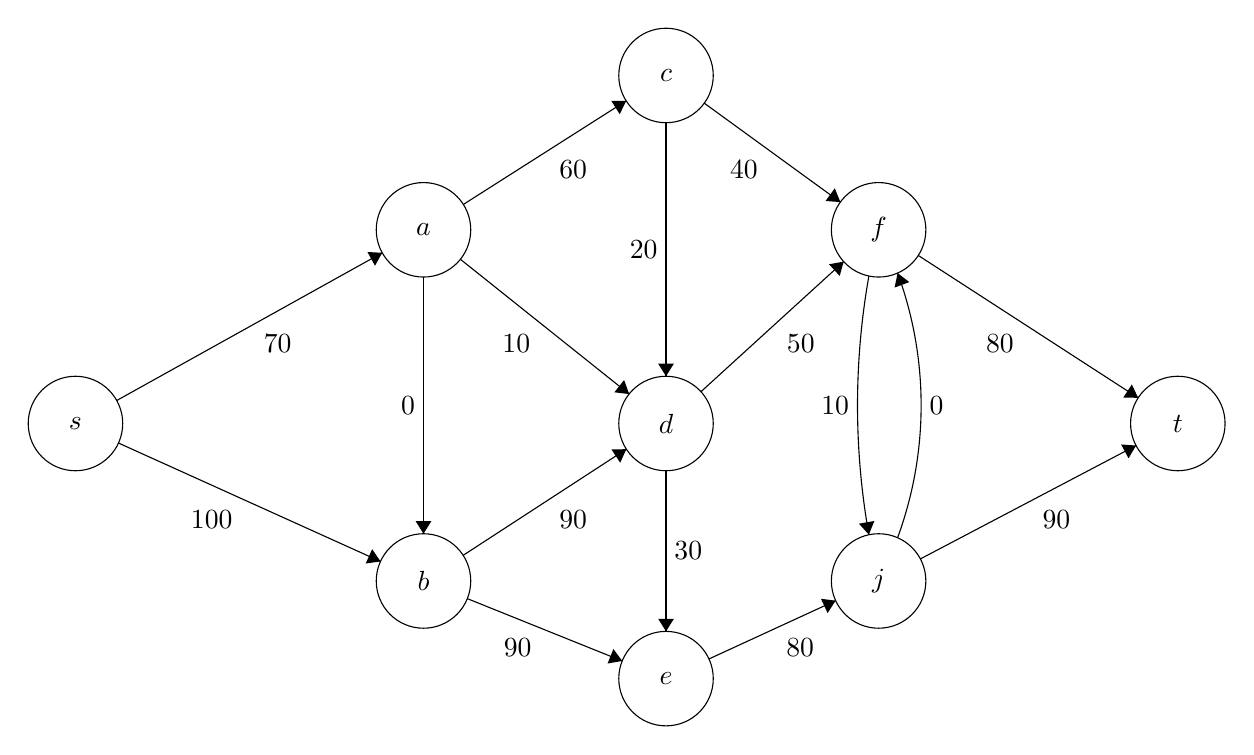
\begin{tikzpicture}[scale=0.2]
	\tikzstyle{every node}+=[inner sep=0pt]
	\draw [black] (4.3,-34.5) circle (3);
	\draw (4.3,-34.5) node {$s$};
	\draw [black] (41.8,-12.4) circle (3);
	\draw (41.8,-12.4) node {$c$};
	\draw [black] (26.4,-22.2) circle (3);
	\draw (26.4,-22.2) node {$a$};
	\draw [black] (26.4,-44.5) circle (3);
	\draw (26.4,-44.5) node {$b$};
	\draw [black] (41.8,-34.5) circle (3);
	\draw (41.8,-34.5) node {$d$};
	\draw [black] (41.8,-50.7) circle (3);
	\draw (41.8,-50.7) node {$e$};
	\draw [black] (55.3,-22.2) circle (3);
	\draw (55.3,-22.2) node {$f$};
	\draw [black] (55.3,-44.5) circle (3);
	\draw (55.3,-44.5) node {$j$};
	\draw [black] (74.3,-34.5) circle (3);
	\draw (74.3,-34.5) node {$t$};
	\draw [black] (7.03,-35.74) -- (23.67,-43.26);
	\fill [black] (23.67,-43.26) -- (23.14,-42.48) -- (22.73,-43.39);
	\draw (12.95,-40.02) node [below] {$100$};
	\draw [black] (26.4,-25.2) -- (26.4,-41.5);
	\fill [black] (26.4,-41.5) -- (26.9,-40.7) -- (25.9,-40.7);
	\draw (25.9,-33.35) node [left] {$0$};
	\draw [black] (41.8,-37.5) -- (41.8,-47.7);
	\fill [black] (41.8,-47.7) -- (42.3,-46.9) -- (41.3,-46.9);
	\draw (42.3,-42.6) node [right] {$30$};
	\draw [black] (56.505,-24.945) arc (20.17249:-20.17249:24.372);
	\fill [black] (56.51,-24.95) -- (56.31,-25.87) -- (57.25,-25.52);
	\draw (58.5,-33.35) node [right] {$0$};
	\draw [black] (6.92,-33.04) -- (23.78,-23.66);
	\fill [black] (23.78,-23.66) -- (22.84,-23.61) -- (23.32,-24.48);
	\draw (17.14,-28.85) node [below] {$70$};
	\draw [black] (28.93,-20.59) -- (39.27,-14.01);
	\fill [black] (39.27,-14.01) -- (38.33,-14.02) -- (38.86,-14.86);
	\draw (35.9,-17.8) node [below] {$60$};
	\draw [black] (28.74,-24.07) -- (39.46,-32.63);
	\fill [black] (39.46,-32.63) -- (39.14,-31.74) -- (38.52,-32.52);
	\draw (32.29,-28.84) node [below] {$10$};
	\draw [black] (28.92,-42.87) -- (39.28,-36.13);
	\fill [black] (39.28,-36.13) -- (38.34,-36.15) -- (38.89,-36.99);
	\draw (35.9,-40) node [below] {$90$};
	\draw [black] (29.18,-45.62) -- (39.02,-49.58);
	\fill [black] (39.02,-49.58) -- (38.46,-48.82) -- (38.09,-49.74);
	\draw (32.38,-48.13) node [below] {$90$};
	\draw [black] (44.53,-49.45) -- (52.57,-45.75);
	\fill [black] (52.57,-45.75) -- (51.64,-45.63) -- (52.06,-46.54);
	\draw (50.32,-48.11) node [below] {$80$};
	\draw [black] (44.02,-32.48) -- (53.08,-24.22);
	\fill [black] (53.08,-24.22) -- (52.15,-24.39) -- (52.83,-25.13);
	\draw (50.36,-28.84) node [below] {$50$};
	\draw [black] (44.23,-14.16) -- (52.87,-20.44);
	\fill [black] (52.87,-20.44) -- (52.52,-19.56) -- (51.93,-20.37);
	\draw (46.75,-17.8) node [below] {$40$};
	\draw [black] (41.8,-15.4) -- (41.8,-31.5);
	\fill [black] (41.8,-31.5) -- (42.3,-30.7) -- (41.3,-30.7);
	\draw (41.3,-23.45) node [left] {$20$};
	\draw [black] (57.82,-23.83) -- (71.78,-32.87);
	\fill [black] (71.78,-32.87) -- (71.38,-32.02) -- (70.84,-32.85);
	\draw (63,-28.85) node [below] {$80$};
	\draw [black] (54.682,-41.565) arc (-169.9437:-190.0563:47.045);
	\fill [black] (54.68,-41.56) -- (55.03,-40.69) -- (54.05,-40.86);
	\draw (53.46,-33.35) node [left] {$10$};
	\draw [black] (57.95,-43.1) -- (71.65,-35.9);
	\fill [black] (71.65,-35.9) -- (70.7,-35.83) -- (71.17,-36.71);
	\draw (66.59,-40.01) node [below] {$90$};
	\end{tikzpicture}
\end{center}

$\rightarrow$ Max Flow: $170$


\section*{Aufgabe 5}
\subsection*{a)}
Zu Beginn, setzen wir für alle Kanten, die Kapazitäten auf 1. Mithilfe des Maxflow Algorithmus (Ford-Fulkerson), wie er in Aufgabe 4 verwendet wurde, können wir nun wie in Aufgabe 2 beschrieben und aus dem max-flow min-cut Theorem folgend, den Mincut berchenen. Da wir alle Kanten zuvor auf 1 gesetzt haben, ist der Mincut genau die Zusammenhangszahl des Graphen, da der Mincut genau der Cut ist, der den Graphen in zwei Teile schneidet und exakt der Cut mit geringster Kapazität. Da hier alle Kapazitäten 1 sind ist der Cut also genau der Cut mit der gerinsten Anzahl an Kanten, demnach entspricht der mincut auch der Zusammenhangszahl.



\subsection*{b)}
\begin{lstlisting}
	function zusammenhangszahl(graph):
		
		# set capacities to 1
		for e in graph.edeges:
			e.weight = 1
		
		# calculate mincut
		zusammenhangszahl = get_mincut(graph)
		
		return zusammenhangszahl

\end{lstlisting}













\end{document}